\documentclass[tikz,border=12pt]{standalone}
\usepackage[T1]{fontenc}
\usepackage{lmodern}
\usetikzlibrary{arrows.meta,positioning}
\begin{document}
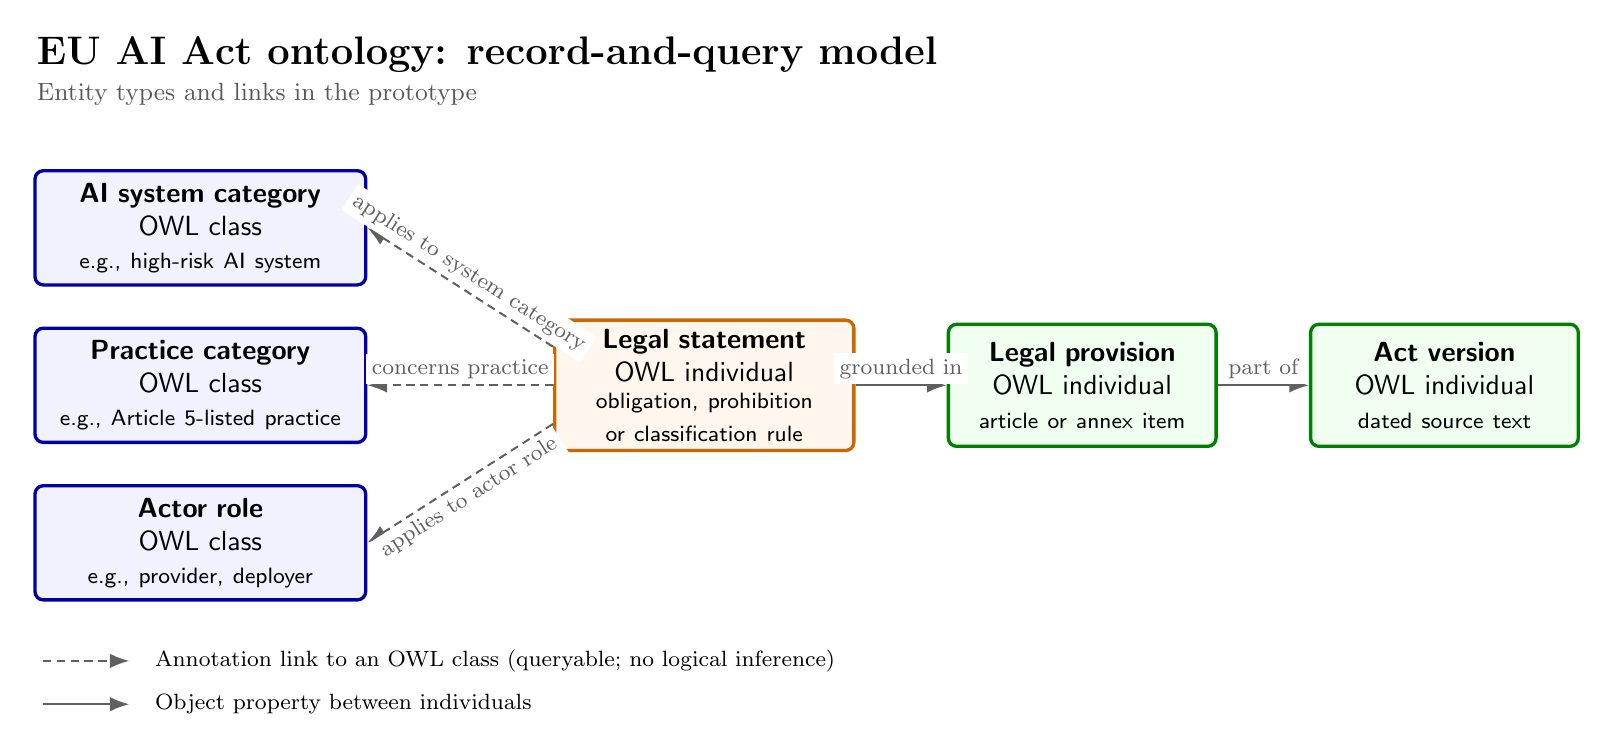
\begin{tikzpicture}[
  font=\sffamily,
  class/.style={draw=blue!65!black,fill=blue!5,rounded corners=3pt,very thick,minimum width=4.2cm,minimum height=1.45cm,align=center,text width=3.95cm},
  norm/.style={draw=orange!80!black,fill=orange!7,rounded corners=3pt,very thick,minimum width=3.8cm,minimum height=1.65cm,align=center,text width=3.5cm},
  source/.style={draw=green!50!black,fill=green!6,rounded corners=3pt,very thick,minimum width=3.4cm,minimum height=1.55cm,align=center,text width=3.15cm},
  annot/.style={-{Latex[length=2.5mm]},densely dashed,thick,gray!75!black},
  object/.style={-{Latex[length=2.5mm]},thick,gray!75!black},
  edge/.style={font=\footnotesize,fill=white,inner sep=2pt,align=center}
]
\node[font=\Large\bfseries,anchor=west] at (-2.2,6.2) {EU AI Act ontology: record-and-query model};
\node[font=\small,anchor=west,text=gray!70!black] at (-2.2,5.7) {Entity types and links in the prototype};

\node[class] (system) at (0,4.0) {\textbf{AI system category}\\OWL class\\\footnotesize e.g., high-risk AI system};
\node[class] (practice) at (0,2.0) {\textbf{Practice category}\\OWL class\\\footnotesize e.g., Article 5-listed practice};
\node[class] (actor) at (0,0.0) {\textbf{Actor role}\\OWL class\\\footnotesize e.g., provider, deployer};

\node[norm] (norm) at (6.4,2.0) {\textbf{Legal statement}\\OWL individual\\\footnotesize obligation, prohibition\\or classification rule};
\node[source] (provision) at (11.2,2.0) {\textbf{Legal provision}\\OWL individual\\\footnotesize article or annex item};
\node[source] (version) at (15.8,2.0) {\textbf{Act version}\\OWL individual\\\footnotesize dated source text};

\draw[annot] ([yshift=14pt]norm.west) -- node[edge,above,sloped] {applies to system category} (system.east);
\draw[annot] (norm.west) -- node[edge,above] {concerns practice} (practice.east);
\draw[annot] ([yshift=-14pt]norm.west) -- node[edge,below,sloped] {applies to actor role} (actor.east);
\draw[object] (norm.east) -- node[edge,above] {grounded in} (provision.west);
\draw[object] (provision.east) -- node[edge,above] {part of} (version.west);

\draw[annot] (-2.0,-1.5) -- (-0.9,-1.5);
\node[anchor=west,font=\footnotesize] at (-0.7,-1.5) {Annotation link to an OWL class (queryable; no logical inference)};
\draw[object] (-2.0,-2.05) -- (-0.9,-2.05);
\node[anchor=west,font=\footnotesize] at (-0.7,-2.05) {Object property between individuals};
\end{tikzpicture}
\end{document}
